
Science is understanding the world -- $\theta \epsilon \omega \rho \iota \alpha $; art is affecting the world -- $ \pi \rho \alpha \xi \iota \sigma $.
Outreach for scientists is a matter not just of connecting with colleagues in the academy, as C.P. Snow~\cite{SnowTwoCultures} said, bridging the Two Cultures.
It is reaching back to our innate humanity and the world from which it came, the universe trying to understand itself. 
No single exhibit reaches this goal, though we do our best with rubber sheets, lasers, and interactive light and sound sculptures. 
Diligence nonetheless can spark curiosity.
LIGO has made concerted efforts to reach further into the universe with ever more sensitive technology, and in leadup to the World Science Festival exhibit on LIGO in 2010 in Manhattan, we tenaciously developed more sophisticated exhibits to connect with a broader audience. 

    \section{Prototypes: travelling kiosks and the Ann Arbor Hands-On Museum} 
    \label{prototypes}

        Prototypes: Ann Arbor Hands-On Museum and travelling kiosk.

    \section{World Science Festival interferometer manufacture}
    \label{manufacture}

        World Science Festival interferometer in isolation.

        \subsection{Laser, optics and display}
        \label{laser_display}

            Laser and optics (and display).

	\begin{figure}
	\begin{center}
	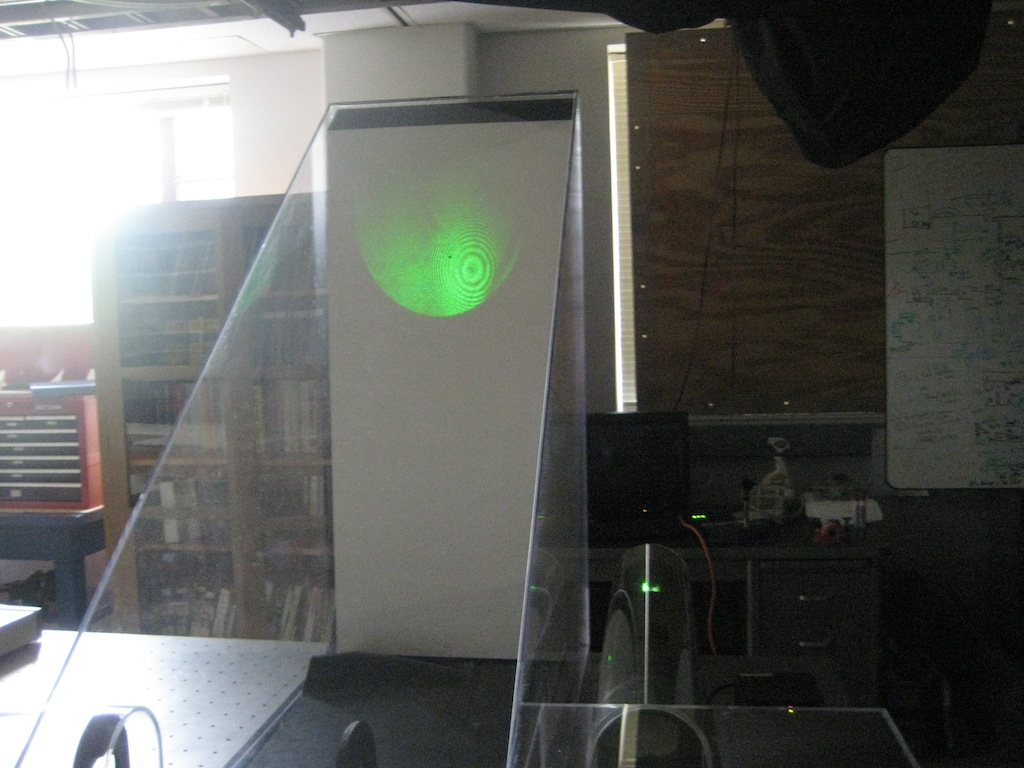
\includegraphics[height=120mm, width=160mm]{WSF_AA_fringes.eps}
	\caption{Interferometer fringes during construction in Ann Arbor}
	\label{WSF_AA_fringes}
	\end{center}
	\end{figure}


        \subsection{Aluminum baseboard}
        \label{baseplate}

            Aluminum base plate.

        \subsection{Plexiglass enclosure}
        \label{enclosure}

            Plexiglass, many lessons learned.

	\begin{figure}
	\begin{center}
	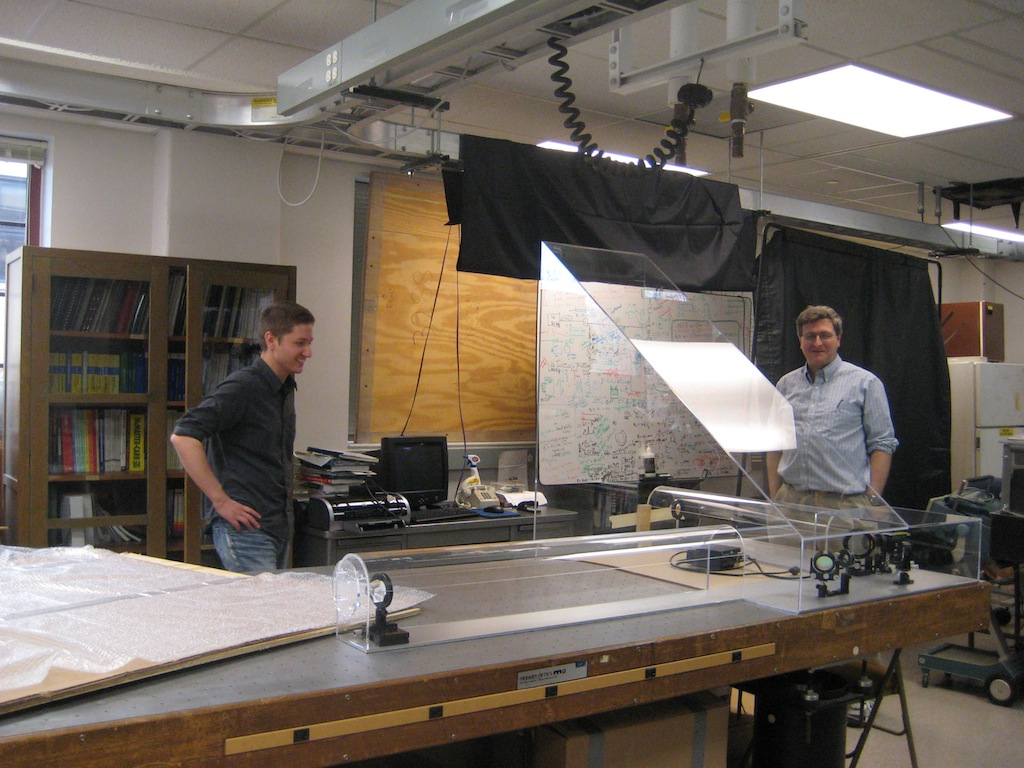
\includegraphics[height=120mm, width=160mm]{WSF_under_construction.eps}
	\caption{Inteferometer assembly in Ann Arbor, Michigan}
	\label{WSF_in_AA}
	\end{center}
	\end{figure}


    \section{Exhibitions: New York City, Portsmouth, Fort Wayne}
    \label{exhibitions}

        World Science Festival interferometer installed.

	\begin{figure}
	\begin{center}
	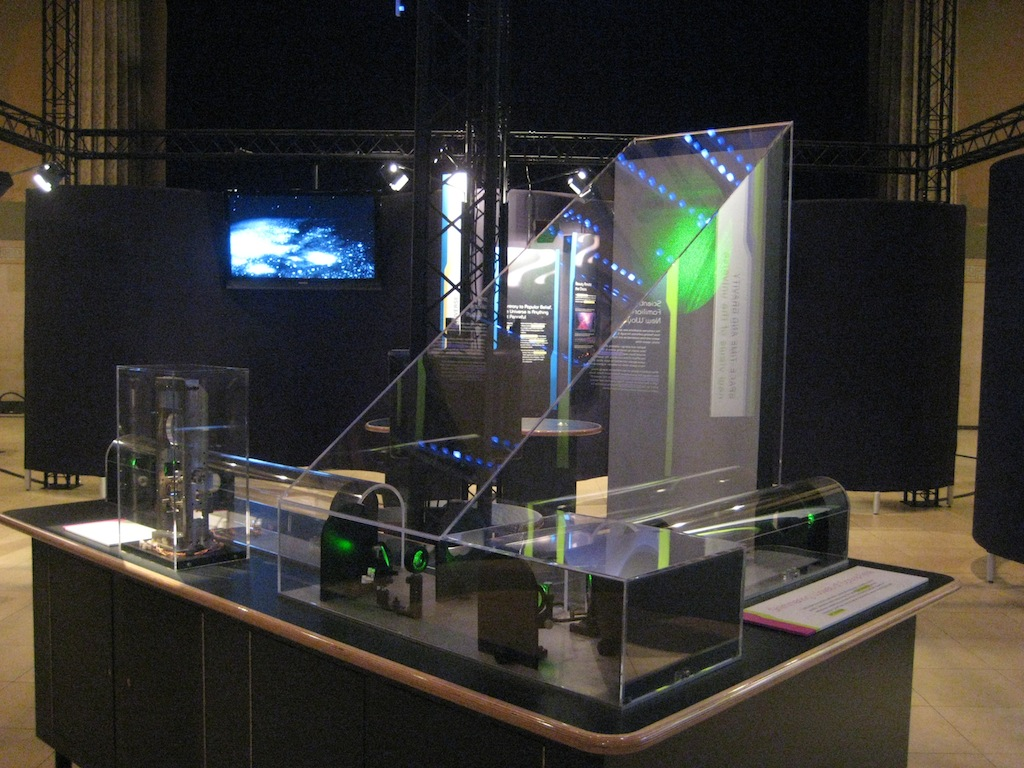
\includegraphics[height=120mm, width=160mm]{WSF_in_NY.eps}
	\caption{World Science Festival interferometer installed in the New York City exhibition hall, June 2010.}
	\label{WSF_IFO_photo}
	\end{center}
	\end{figure}


        \subsection{Exhibit overview}
        \label{exhibit_overview}

            NYC exhibit overview: design, walls, kiosks, displays, interactivities.

        \subsection{World Science Festival 2010}
        \label{WSF2010}

            Success in WSF 2010.

	\begin{figure}
	\begin{center}
	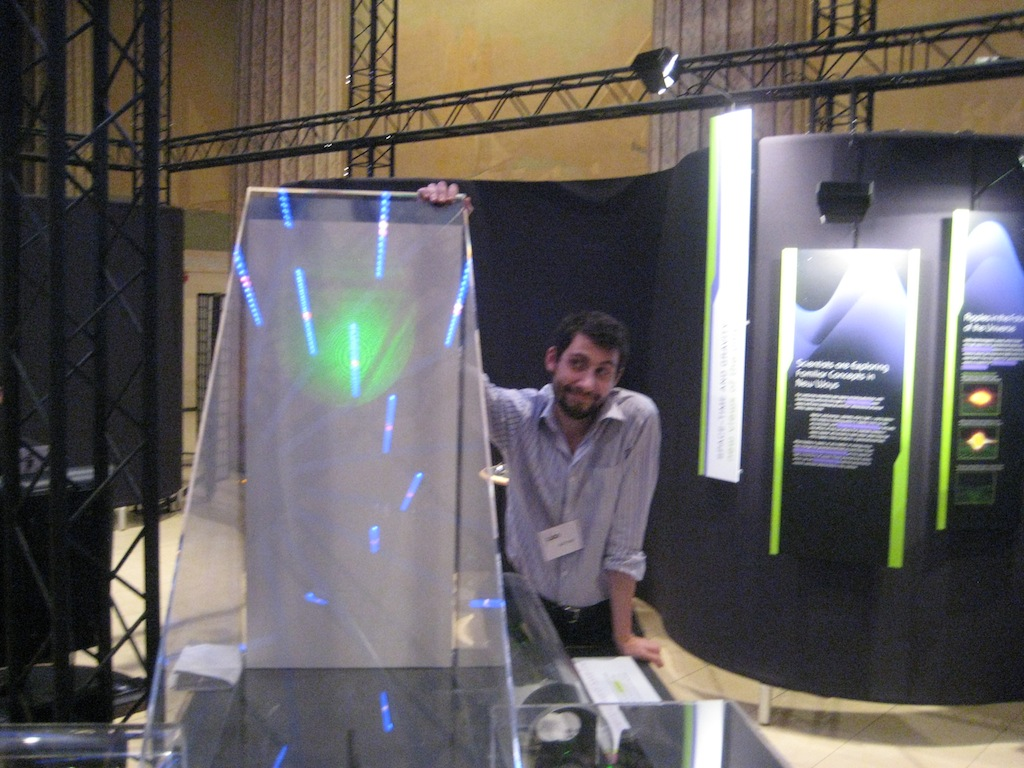
\includegraphics[height=120mm, width=160mm]{WSF_me_NY.eps}
	\caption{Helping to host the exhibit at the World Science Festival.}
	\label{WSF_IFO_me}
	\end{center}
	\end{figure}


        \subsection{Portsmouth and Fort Wayne}
        \label{secondary_installations}

            Secondary installations and future outreach potential.

    \section{Future LIGO outreach}
    \label{future_outreach}

        Epilogue: as of June 2014, the exhibit is safely on display in the Livingston Science and Education center.

        Future LIGO outreach? How to explain a new astronomy.


        --------------------------------------

	%The following is an example of using the commands \textit{ref}
	%and \textit{label}. With these commands theorems, chapters,
	%sections and figurres can be labeld with names in the tex file
	%and then refered to by these names in later tex files. In
	%chapter~\ref{intro} we saw section~\ref{sample_section} or
	%theorem~\ref{sample_theorem}.

	%Lastly, here is how to include a figure. First generate an
	%encapsulated postscript file in xfig, adobe illustrator or
	%some other program. The specific commands are found in
	%\textit{chap2.tex}.

        %\begin{figure}[htb]
        %\centerline{ \epsfig{figure=sample.eps, 
        %height =  1.5 in}}
        %\caption{Sample Figure}
        %\label{sample_figure}
        %\end{figure}

